\begin{center}
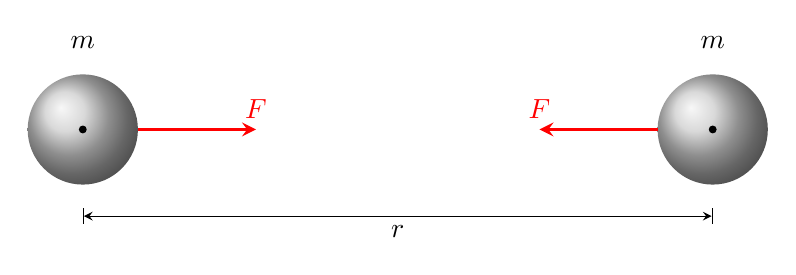
\begin{tikzpicture}[>=stealth]
 \shade[ball color=gray!40] (0,0) circle (0.7);
 \shade[ball color=gray!40] (8,0) circle (0.7);
 \fill (0,0) circle (0.05);
 \fill (8,0) circle (0.05);
 \node at (0,1.1) {$m$};
 \node at (8,1.1) {$m$};
 \draw[->, very thick, red] (0.7,0) -- (2.2,0) node[above] {$F$};
 \draw[->, very thick, red] (7.3,0) -- (5.8,0) node[above] {$F$};
 \draw[|<->|] (0,-1.1) -- (8,-1.1) node[midway, below] {$r$};
\end{tikzpicture}
\end{center}

Homogene Kugeln ziehen sich an wie Punktmassen in ihren Mittelpunkten. Beim Abstand $r_1 = \rAO$ ist
\begin{align}
 F_1 &= \FAF \\
   &= \ncG\cdot\frac{\left(\mKu\right)^2}{\left(\rA\right)^2} \\
   &= \FA \approx \result{\FAP{-9}{2}}
\end{align}
Die Kraft ist umgekehrt proportional zum Quadrat des Abstands. Beim halben Abstand $r_2 = \rBO$ ist sie viermal so gross:
\begin{align}
 F_2 &= \FBF = F_1\cdot 2^2 = \FB \approx \result{\FBP{-9}{2}}
\end{align}
Beim fünffachen Abstand $r_3 = \rCO$ ist sie 25-mal kleiner:
\begin{align}
 F_3 &= \FCF = \frac{F_1}{5^2} = \FC \approx \result{\FCP{-9}{2}}
\end{align}
